\documentclass[tikz]{standalone}
\usepackage{amsmath}
\definecolor{bg}{HTML}{171D2B}
\definecolor{aksen}{HTML}{F7B538}
\definecolor{teks}{HTML}{FFFFFF}
\definecolor{isi}{HTML}{64748B}
\pagecolor{bg}
\begin{document}
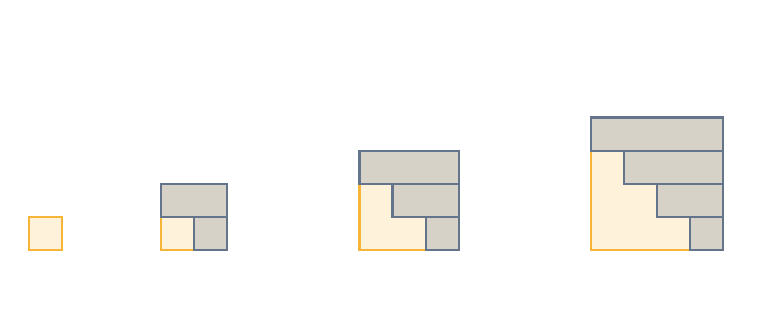
\begin{tikzpicture}[scale=0.42,
  kuadrat/.style={draw=aksen, fill=aksen, fill opacity=0.18, line width=0.8pt},
  tambah/.style={draw=isi, fill=isi, fill opacity=0.25, line width=0.8pt},
  lbl/.style={teks, font=\small}]
% Persegi 1 : 1 titik, tanpa lapisan tambahan
\draw[kuadrat] (0,0) rectangle (1,1);
% Persegi 2 : + lapisan sisi kanan & atas (3 titik)
\draw[kuadrat] (4,0) rectangle (6,2);
\draw[tambah] (5,0) rectangle (6,1);
\draw[tambah] (4,1) rectangle (6,2);
% Persegi 3 : + lapisan (5 titik)
\draw[kuadrat] (10,0) rectangle (13,3);
\draw[tambah] (12,0) rectangle (13,1);
\draw[tambah] (11,1) rectangle (13,2);
\draw[tambah] (10,2) rectangle (13,3);
% Persegi 4 : + lapisan (7 titik)
\draw[kuadrat] (17,0) rectangle (21,4);
\draw[tambah] (20,0) rectangle (21,1);
\draw[tambah] (19,1) rectangle (21,2);
\draw[tambah] (18,2) rectangle (21,3);
\draw[tambah] (17,3) rectangle (21,4);
% label jumlah titik
\node[lbl, anchor=south] at (0.5,1.15) {1};
\node[lbl, anchor=south] at (5,2.15) {4};
\node[lbl, anchor=south] at (11.5,3.15) {9};
\node[lbl, anchor=south] at (19,4.15) {16};
% panah jumlah lapisan
\node[lbl, anchor=north, font=\footnotesize] at (5,-0.35) {$1+3$};
\node[lbl, anchor=north, font=\footnotesize] at (11.5,-0.35) {$1+3+5$};
\node[lbl, anchor=north, font=\footnotesize] at (19,-0.35) {$1+3+5+7$};
\node[lbl, anchor=south, font=\normalsize\bfseries] at (10,5.4) {Pola Bilangan Persegi};
\end{tikzpicture}
\end{document}